A transformação energética é fundamental ao projeto, é a partir dela que é proporcionado o funcionamento integral dos componentes da turbina afim de se captar a água do ar. Dentre as formas de energia utilizadas, a energia inicial é a contida nos ventos, fonte primária que alimentará todo o sistema. 

A força dos ventos ao entrar em contato com as pás do rotor, e devido a forma aerodinâmica das pás, faz com que haja rotação do mesmo. Para garantir a produção de energia, é necessário que os ventos possuam uma velocidade mínima suficiente para o funcionamento do sistema.  Ligado ao rotor, existe um eixo mecânico. Esse eixo mecânico é dividido em duas partes, uma de baixa velocidade e uma de alta velocidade. A função dos dois eixos é garantir um maior aproveitamento da energia de rotação do rotor transmitindo energia do eixo de baixa rotação para o eixo de alta rotação sendo estes interligados através da caixa multiplicadora. A função da caixa multiplicadora é multiplicar a rotação angular em relação ao eixo de baixa rotação e ao de alta rotação, atingindo assim nível necessário de rotação no gerador. Essa rotação das pás gira o eixo mecânico, que por sua vez está ligado ao gerador elétrico. Deste modo, temos a conversão da energia cinética dos ventos em energia mecânica de rotação através do eixo do rotor. Por fim, o gerador  converte a energia mecânica de rotação proveniente do eixo mecânico em energia elétrica. 

Para o rotor, considera-se o número de pás, desempenho aerodinâmico, materiais e o controle da rotação afim de evitar danos ao equipamento. A caixa multiplicadora uni os dois eixos a partir de engrenagens com o intuito de aumentar a velocidade da rotação angular, devido ao fato da rotação das pás ser baixa e o gerador exigir rotações maiores. A energia produzida é do tipo corrente alternada, pelo fato do gerador elétrico ser do tipo de indução, assíncrono, composto de estator e rotor, trifásico, o que facilita a distribuição direta aos componentes da turbina eólica. A tensão e a frequência de saída são controladas por uma unidade de condicionamento de potência que é definida de acordo com a necessidade dos equipamentos presentes na turbina eólica.

No caso do armazenamento em baterias, uma conversão para corrente continua é necessária. Essa conversão é feita por um conversor presente na torre de controle onde estarão as baterias.  As baterias utilizadas no projeto serão do tipo baterias estacionárias moura clean 220Ah, resistentes a altas temperaturas e dispensam a necessidade de resfriamento do ambiente. De acordo com o fabricante, são baterias ecoeficientes e estão de acordo com a regulamentação do CONAMA, além de serem indicadas para o armazenamento de energia de fontes renováveis. As baterias serão dispostas em uma sala para o seu armazenamento e utilizadas somente em caso de emergência. 

A seguir é apresentado o diagrama esquemático do caminho energético:
\begin{figure}[!ht]
\centering
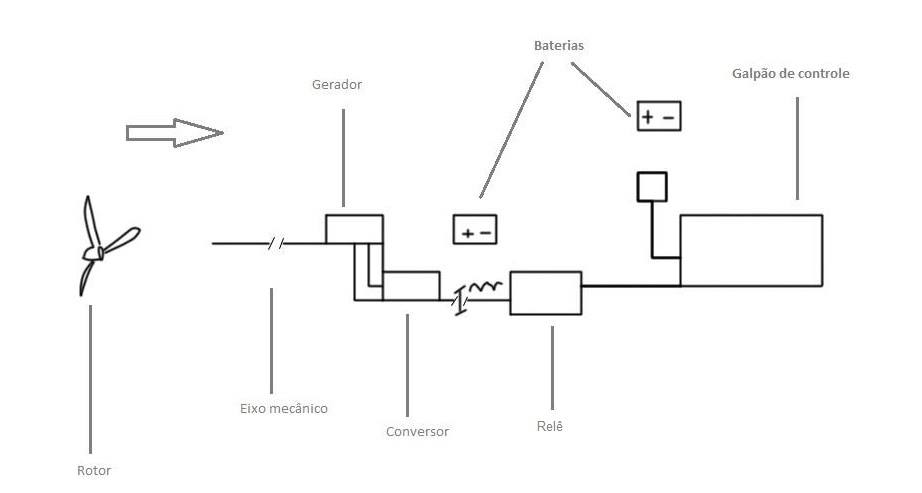
\includegraphics[scale=0.5]{editaveis/figuras/diagrama_energetico}
\caption[Diagrama energético]{Diagrama esquemático do caminho energético}
\label{energertico}
\end{figure}
\FloatBarrier